\begingroup
% Shared visual language for the three segmentation-method diagrams.
\tikzset{
    box/.style={draw, rounded corners=2pt, align=center, font=\small,
        text width=44mm, minimum height=9mm, inner sep=4pt, line width=0.5pt},
    process/.style={box, fill=gray!7},
    model/.style={box, very thick, fill=blue!5},
    output/.style={box, dashed},
    supervision/.style={box, densely dashed, fill=gray!7},
    link/.style={->, semithick},
    traininglink/.style={link, densely dashed}
}

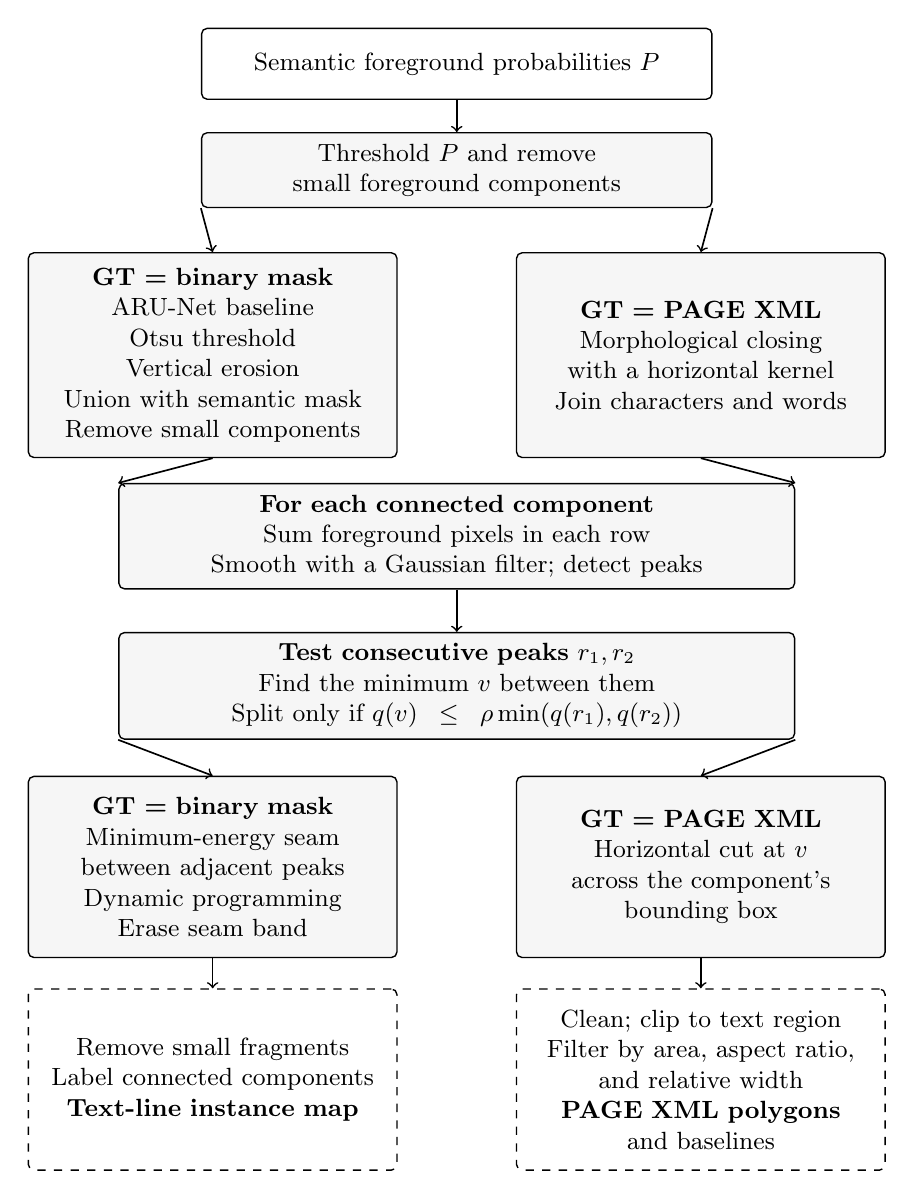
\begin{tikzpicture}
    \node[box, text width=62mm] (input) at (0,0)
        {Semantic foreground probabilities \(P\)};
    \node[process, text width=62mm] (clean) at (0,-1.35)
        {Threshold \(P\) and remove\\small foreground components};
    \node[process, minimum height=26mm] (binary-prep) at (-3.1,-3.7)
        {\textbf{GT = binary mask}\\ARU-Net baseline\\Otsu threshold\\Vertical erosion\\Union with semantic mask\\Remove small components};
    \node[process, minimum height=26mm] (xml-prep) at (3.1,-3.7)
        {\textbf{GT = PAGE XML}\\Morphological closing\\with a horizontal kernel\\Join characters and words};
    \node[process, text width=83mm] (projection) at (0,-6.0)
        {\textbf{For each connected component}\\Sum foreground pixels in each row\\Smooth with a Gaussian filter; detect peaks};
    \node[process, text width=83mm] (valley) at (0,-7.9)
        {\textbf{Test consecutive peaks \(r_1,r_2\)}\\Find the minimum \(v\) between them\\Split only if \(q(v)\leq\rho\min(q(r_1),q(r_2))\)};
    \node[process, minimum height=23mm] (seam) at (-3.1,-10.2)
        {\textbf{GT = binary mask}\\Minimum-energy seam\\between adjacent peaks\\Dynamic programming\\Erase seam band};
    \node[process, minimum height=23mm] (cut) at (3.1,-10.2)
        {\textbf{GT = PAGE XML}\\Horizontal cut at \(v\)\\across the component's\\bounding box};
    \node[output, minimum height=23mm] (binary-out) at (-3.1,-12.9)
        {Remove small fragments\\Label connected components\\\textbf{Text-line instance map}};
    \node[output, minimum height=23mm] (xml-out) at (3.1,-12.9)
        {Clean; clip to text region\\Filter by area, aspect ratio,\\and relative width\\\textbf{PAGE XML polygons}\\and baselines};
    \draw[link] (input) -- (clean);
    \draw[link] (clean.south west) -- (binary-prep.north);
    \draw[link] (clean.south east) -- (xml-prep.north);
    \draw[link] (binary-prep.south) -- (projection.north west);
    \draw[link] (xml-prep.south) -- (projection.north east);
    \draw[link] (projection) -- (valley);
    \draw[link] (valley.south west) -- (seam.north);
    \draw[link] (valley.south east) -- (cut.north);
    \draw[link] (seam) -- (binary-out);
    \draw[link] (cut) -- (xml-out);
\end{tikzpicture}
\endgroup
